\section{Systeem}
Het volledige systeem bestaat uit twee verschillende onderdelen: een aantal sensor nodes en een basisstation node.
De sensor nodes verzamelen data van een sensor, en sturen dit naar de basisstation node. De basisstation node verzamelt al deze data, en toont het op een scherm. Op het scherm worden ook eventuele metaconclusies getoond.
De nodes communiceren met elkaar over een dynamisch draadloos sensor netwerk (DWSN).
Dit is een netwerk dat een variabel aantal nodes kan bevatten, die allemaal verplaatst mogen worden. Nodes in een DWSN kunnen automatisch verbinding maken met het netwerk.

Er is gekozen voor een DWSN door de flexibiliteit. Nodes kunnen met gemak verplaatst, toegevoegd of verwijderd worden. Het netwerk is zo ontworpen dat er meerdere verschillende systemen in kunnen werken, zonder dat deze  elkaar storen.

\begin{figure}[ht]
    \centering
    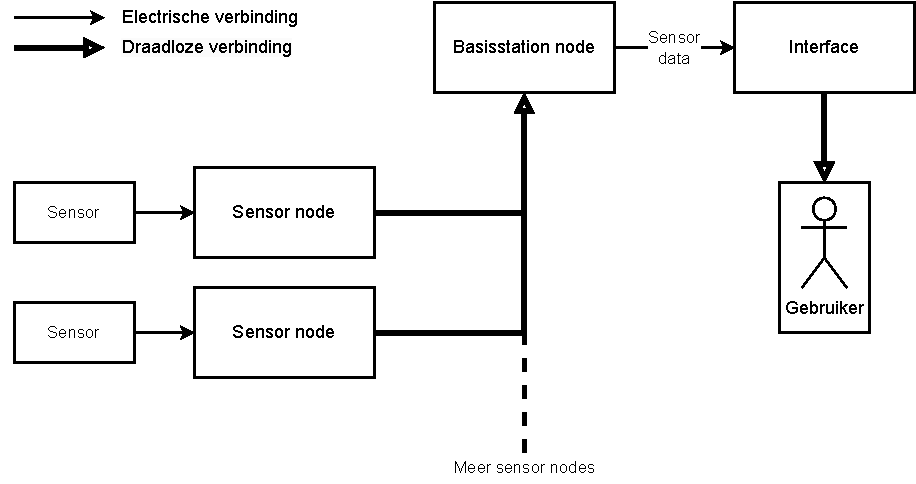
\includegraphics{img/fullsystem.pdf}
    \caption{Een blokschema van het systeem.}
    \label{fig:fullsystem}
\end{figure}

\subsection{Specificaties}

In \autoref{tab:grootheden} zijn de gemeten grootheden te zien.
De sensornodes sturen de gemeten waardes elke seconde op. 

\begin{table}[ht]
    \centering
    \begin{tabular}{l||l|l|l}
        & Eenheid & Meetbereik\\
        \hline
        Luchtvochtigheid & \%          & 0 tot 100\%           & \cite{palonen1993effects}  \\
        Temperatuur      & $^{\circ}$C & 10 tot 30 $^{\circ}$C & \cite{palonen1993effects}  \\
        VOC's            & \(mg/m^3\)  & 10 \(mg/m^3\)         & \cite{voc-luchtkwaliteit}  \\
        Geluidsniveau    & dBA         & 50 - 80dBA            & \cite{geluid-levels}       \\
        Licht            & Lx          & 0 - 1000 Lx           & \cite{lightingIndorWorkspaces}
    \end{tabular}
    \caption{De gemeten grootheden.}
    \label{tab:grootheden}
\end{table}

 